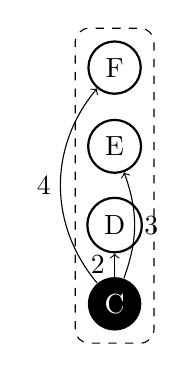
\begin{tikzpicture}
    \node (bottom) at (0,0) [circle, fill=black, text=white, minimum width=1.5em] {C};
    \node (top1) at (0, 1) [circle, draw=black, thick, minimum width=1.5em] {D};
    \node (top2) at (0, 2) [circle, draw=black, thick, minimum width=1.5em] {E};
    \node (top3) at (0, 3) [circle, draw=black, thick, minimum width=1.5em] {F};
    \draw[rounded corners=5pt, dashed] (-0.5, -0.5) rectangle (0.5, 3.5);
    % Draw curved arrows with annotations
    \draw[->, bend left=0] (bottom) to node[midway, left] {2} (top1);
    \draw[->, bend right=20] (bottom) to node[midway, right] {3} (top2);
    \draw[->, bend left=40] (bottom) to node[midway, left] {4} (top3);
\end{tikzpicture}
